\documentclass{scrartcl}
\usepackage{vmargin}
\usepackage{amssymb}
\usepackage{amsmath}
\usepackage{amsthm}
\usepackage{pgfplots} 
\usepackage{graphicx}
\usepackage[utf8x]{inputenc}
\usepackage{tikz}
\usepackage{bbm}
\usepackage{subcaption}
\usepackage[boxruled]{algorithm2e}
\usepackage{mathtools}
\usepackage[toc,page]{appendix}
\DeclarePairedDelimiter{\ceil}{\lceil}{\rceil}
\newcommand{\eqtext}[1]{\ensuremath{\stackrel{#1}{=}}}
\newtheorem{theorem}{Proposition}[section]
\newtheorem{lemma}{Lemma}[section]
\newtheorem{remark}{Remark}[section]
\newcommand{\N}{\mathbb{N}}
\newcommand{\R}{\mathbb{R}}
\newcommand{\E}{\mathbb{E}}
\newcommand{\epl}{\epsilon}

\title{Uncertain Darcy's problem and the stochastic particle transport}

\author{Giacomo Garegnani \\ {Supervisors: Dr. Sebastian Krumscheid and Prof. Fabio Nobile}}
\date{}

\begin{document}
\maketitle
\tableofcontents
\newpage
\section{Expected exit time from a domain}
We aim to estimate the exit time of a particle driven by a deterministic transport field and a stochastic diffusion from a domain $D \subset \mathbb{R}^d$. Given a vector $W(t)$ of $m$ independent Brownian motions and two functions $f\colon \mathbb{R}^d \rightarrow \mathbb{R}^d, g \colon \mathbb{R}^d \rightarrow \mathbb{R}^{d\times m}$, we consider the following stochastic differential equation (SDE)
\begin{equation}\label{eq:GeneralModel}
\begin{cases}
	dX(t) = f(X(t)) dt + g(X(t))dW(t), & 0 < t \leq T, \\
	X(0)  = X_0, & X_0 \in D.
\end{cases}
\end{equation}
The problem is completed with two different types of boundary conditions, namely
\begin{itemize}
	\item[i.]  \textit{killing boundaries}: if the particle exits $D$ the process is stopped,
	\item[ii.] \textit{reflecting boundaries}: the particle trajectory is reflected normally inside $D$ when it touches the boundary $\partial D$.
\end{itemize}
Our aim is to estimate numerically the first exit time of the solution $X(t)$ from $D$, \textit{i.e.}, the quantity
\begin{equation}\label{eq:GeneralTau}
	\tau = \min\{\min\{t\colon X(t)\notin D\},T\}.
\end{equation}
Let us remark that the parameter $\tau$ is meaningful only if there exists a portion of the boundary $\Gamma_k \subset \partial D$ that is endowed with killing boundary conditions. Otherwise, the process $X(t)$ will stay in $D$ for the whole time interval, giving as a result $\tau = T$ for each realisation of $X(t)$. Another quantity of interest is defined as follows
\begin{equation}\label{eq:GeneralPhi}
	\phi = \mathbbm{1}_{\{\tau<T\}}F(X(T)),
\end{equation}
where $F\colon \mathbb{R}^d \rightarrow \mathbb{R}$ is a smooth function. An interesting choice of $F$ could be the identity function, thus giving as a result for $\phi$ the probability for $X(t)$ to exit the domain before the final time $T$, \textit{i.e.}, 
\begin{equation}\label{eq:ExitProb}
	\phi \eqtext{\{F\equiv0\}} \Pr(\tau < T | X(0) = X_0)
\end{equation}
In the case of general $f,g$ and for a $d$-dimensional SDE, there is no closed form for $\tau$ and $\phi$. Therefore, we approximate the value of $\tau$ by means of two numerical schemes, briefly presented in the following.

\subsection{A PDE approach}\label{sec:PDEs}
It is possible to express the mean exit time and the probability of exit from a domain in terms of the solution of partial differential equations (PDE's).
Let us denote by $\Gamma_k,\Gamma_r$ the killing and reflecting subsets of $\partial D$. We consider then the expectation of the exit time from the domain $D$ for a trajectory that at $t=0$ is at position $x$, \textit{i.e.},
\begin{equation}\label{eq:ExpTau}
	\bar\tau(x) = \mathbb{E}(\tau | X(0) = x).
\end{equation}
Let us define the operator $\mathcal L$ induced by \eqref{eq:GeneralModel}, which is applied to a function $u\colon \mathbb{R}^d \rightarrow \mathbb{R}$  as follows
\begin{equation}\label{eq:LOperator}
	\mathcal Lu = f \cdot \nabla u + \frac{1}{2} gg^T : \nabla \nabla u,
\end{equation}
where the $:$ operator between two matrices $A,B$ in $\mathbb{R}^{d\times d}$ is defined as follows
\begin{equation}\label{eq:twoPoints}
	A : B = \sum_{i,j = 1}^d \{A\}_{ij}\{B\}_{ij} = \text{tr}(A^TB).
\end{equation}
The following result allows computing the mean exit time as the solution of an appropriate PDE.

\begin{theorem} Let $\mathcal L$ be the differential operator defined as \eqref{eq:LOperator}. Then, if $\Gamma_k$ and $\Gamma_r$ are respectively the killing and reflecting subsets of $\partial D$, such that $\Gamma_k \cup \Gamma_r = \partial D, \Gamma_k \cap \Gamma_r = \emptyset$, the mean exit time $\bar \tau(x)$ for the solution $X(t)$ of \eqref{eq:GeneralModel} with $X_0 = x$ is the solution of the following boundary value problem
\begin{equation}\label{eq:PDETau}
\left \{
\begin{aligned}
	\mathcal L \bar \tau(x) &= -1, && \text{in } D, \\
	\bar\tau(x) &= 0, && \text{on } \Gamma_k, \\
	\nabla \bar\tau(x) \cdot n &= 0, && \text{on } \Gamma_r,
\end{aligned} \right .
\end{equation}
where $n$ is the normal to $\Gamma_r$.
\end{theorem}
\noindent Further analytic treatment of the mean exit time can be found in \cite{Krumscheid2015,Pavliotis2014}. \\
We now consider the probability of exit from $D$ for a solution $X(t)$ that is equal to $x$ for at a time $s$ smaller than the final time $T$. This probability is the solution of a boundary value problem.
\begin{theorem} Let $\mathcal L$ be the differential operator defined as \eqref{eq:LOperator}. Then, if $\Gamma_k$ and $\Gamma_r$ are respectively the killing and reflecting subsets of $\partial D$, such that $\Gamma_k \cup \Gamma_r = \partial D, \Gamma_k \cap \Gamma_r = \emptyset$
\begin{equation}\label{eq:ExitProbNotation}
	\Pr(\tau < T | X(s) = x) = \Phi(x,s,T) 
\end{equation}
where $\Phi(x,t,T)$ is the solution of the following backwards PDE
\begin{equation}\label{eq:PDEPhi}
\left \{
\begin{aligned}
	\frac{\partial}{\partial t} \Phi(x,t,T) + \mathcal L \Phi(x,t,T) &= 0 && \text{in } D, s \leq t < T, \\
	\Phi(x,t,T) &= 1 && \text{on } \Gamma_k, s \leq t \leq T,\\
	\nabla \Phi(x,t,T) \cdot n &= 0, && \text{on } \Gamma_r, s \leq t \leq T, \\
	\Phi(x,T,T) &= 0 && \text{in } D,
\end{aligned} \right .
\end{equation}
where $n$ is the normal to $\Gamma_r$.
\end{theorem}
\noindent The proof in case $\Gamma_k = \partial D$ of this result can be found in \cite{Sirovich2010}. Further treatment in case of mixed boundary conditions and the closed form of the solution for some particular geometries of $D \subset \mathbb{R}^2$ can be found in \cite{Grebenkov2014}. It is therefore possible to approximate the mean exit time and the exit probability by means of classical methods for solving PDE's numerically, such as finite differences or the Finite Elements Method. In Appendix \ref{sec:Appendix1} we present an analytic formula to compute the mean exit time in the one-dimensional case, and in Appendix \ref{sec:Appendix2} we show a finite difference approach to approximate numerically \eqref{eq:PDETau} in the one-dimensional case. In the two-dimensional case, we solve \eqref{eq:PDETau} and \eqref{eq:PDEPhi} using linear Finite Elements using the PDE toolbox of Matlab.


\begin{frame}[plain]
\frametitle{Discrete Euler-Maruyama}
Method:
\begin{equation*}
	\left \{
	\begin{aligned}
		X_h^d(t_{i+1}) &= f(X(t_i))h + g(X(t_i))(W(t_{i+1}) - W(t_{i})),  \\
		X_h^d(0) &= X_0.
	\end{aligned} \right .
\end{equation*}
Parameters of interest computed naively
\begin{equation*}
\begin{aligned}
	\tau_h^d &= \min\{\tau_{h,e}^d,T\}, \text{ where } \tau_{h,e}^d = \min \{t_i \colon X_h^d(t_i) \notin D\}, \\
	\phi_h^d &= \mathbbm{1}_{\{T < \tau_{h,e}^d\}}F(X_h^d(T)).
\end{aligned}
\end{equation*}
Missed exits $\Rightarrow$ 1/2 loss in weak order:
\begin{align*}
	|\mathbb{E}(\tau_h^d) - \mathbb{E}(\tau)| &= O(\sqrt{h}), \\
	|\mathbb{E}(\phi_h^d) - \mathbb{E}(\phi)| &= O(\sqrt{h}).
\end{align*}	
\end{frame}

\begin{frame}[plain]
\frametitle{Continuous Euler-Maruyama}
\underline{Goal}. Restore the order of convergence 1 of Euler-Maruyama in $\R^d$ $\Rightarrow$ Brownian bridge approach.

Method:
\begin{equation*}
	\left \{
	\begin{aligned}
		X_h^c(t) &= f(X(t_i))(t-t_i) + g(X(t_i))(W(t) - W(t_{i})),  && t_i < t \leq t_{i+1},\\
		X_h^c(0) &= X_0.
	\end{aligned} \right .
\end{equation*} 
Estimate at each time step the probability of exit. If $D$ is an half-space
\begin{equation*}
\begin{aligned}
	&\Pr (\exists t \in [ t_i,t_{i+1} ] \quad X_h^d(t) \notin D | X_h^d(t_i) = x_i, X_h^d(t_{i+1}) = x_{i+1}) \\
	&\quad = p(x_i,x_{i+1},h) \\
	&\quad = \exp\Big(-2\frac{[n\cdot(x_i - z_i)][n\cdot(x_{i+1} - z_i)]}{hn\cdot (gg^T(x_i)n)}\Big),
\end{aligned}
\end{equation*}
\end{frame}

\begin{frame}
\frametitle{Continuous Euler-Maruyama}
Parameters of interest. Given $u$ a realization of $U$ uniform r.v. in $(0,1)$
\begin{equation*}
\begin{aligned}
	\tau_h^c &= \min \{T,\tau_{h,e}^c\}, \\
	\text{ where } \tau_{h,e}^c &= \min\{\tau_{h,e1}^c, \tau_{h,e2}^c\}, \\
	\tau_{h,e1}^c &= \min\{t_i = hi \colon X_h(t_i) \notin D\}, \\
	\tau_{h,e2}^c &= \min\{t_i = hi \colon u < p(x_{i-1},x_i,h) \}, \\
	\phi_h^c &= \mathbbm{1}_{\{T < \tau_{h,e}^c\}}F(X_h^c(T)).
\end{aligned}
\end{equation*}
Weak order 1 is restored:
\begin{align*}
	|\mathbb{E}(\tau_h^c) - \mathbb{E}(\tau)| &= O(h), \\
	|\mathbb{E}(\phi_h^c) - \mathbb{E}(\phi)| &= O(h).
\end{align*}
\end{frame}

\subsection{One-Dimensional Case}
We consider problem \eqref{eq:GeneralModel} in case $d = 1$. Given $f,g$ defined on an interval $D = \left[l,r\right]$ and a Brownian motion $W(t)$, let us consider the following one dimensional SDE
\begin{equation}\label{eq:OneDModel}
\left \{
\begin{aligned}
	dX(t) &= f(X(t)) dt + g(X(t))dW(t), && 0 < t \leq T, \\
	X(0)  &= X_0, && X_0 \in D.
\end{aligned} \right .
\end{equation}
In this case, the boundary of $D$ consists of the two points $\{l,r\}$. In order for the problem of the determination of $\tau$ to be meaningful, at least one of the two points should be endowed with a killing boundary condition. 
\subsubsection{Analytical expression of the mean exit time}
In this simple frame, it is possible to deduce an analytical solution $\bar\tau$ of \eqref{eq:PDETau}. Let us consider the boundary condition at $x=l$ fixed as \textit{killing} and vary the boundary condition at $x=r$. Since the scope is deducing the exit time of a particle from $D$, this assumption is plausible. In this frame, it is possible to rewrite \eqref{eq:PDETau} as
\begin{equation}\label{eq:ODETau}
\left \{
\begin{aligned}
	f(x)\bar\tau'(x) + \frac{1}{2} g^2(x) \bar\tau''(x) &= -1, && l < x < r, \\
	\bar\tau(l) &= 0, \\
	\bar\tau(r) &= 0, && \text{if for $x = r$ the boundary is \textit{killing}}, \\
	\bar\tau'(r) &= 0, && \text{if for $x = r$ the boundary is \textit{reflecting}}. 
\end{aligned} \right .
\end{equation}
It is possible to show \cite{Krumscheid2015,Pavliotis2014} that $\bar\tau$ is in the one-dimensional case given by
\begin{equation}\label{eq:AnalyticTau}
	\bar\tau(x) = -2 \int_l^x \exp(-\psi(z)) \int_l^z \frac{\exp(\psi(y))}{g^2(y)}dy + c_1 \int_l^x \exp(-\psi(y))dy + c_2,
\end{equation}
where the function $\psi$ is defined as
\begin{equation}\label{eq:psi}
	\psi(x) = \int_l^x \frac{2f(y)}{g^2(y)}dy,
\end{equation}
and the constants $c_1,c_2 \in \mathbb{R}$ depend on the boundary conditions as follows
\begin{equation}\label{eq:Constants}
\begin{aligned}
	c_1 &= 2\frac{\int_l^r \exp(-\psi(z)) \int_l^z \frac{\exp(\psi(y))}{g^2(y)}dy}{\int_l^r \exp(-\psi(y))dy}, && \text{  if for $x = r$ the boundary is \textit{killing}}, \\
	c_1 &= 2\int_l^r \frac{\exp(-\psi(y))}{g(y)^2}dy, && \text{  if for $x = r$ the boundary is \textit{reflecting}}, \\
	c_2 &= 0.
\end{aligned}
\end{equation}
Let us remark that in case $f = -V'$ for some smooth function $V$ and $g = \sigma \in \mathbb{R}$, the expression of $\psi$ semplifies to
\begin{equation}\label{eq:psiSemplified}
	\psi(x) = 2\frac{V(l)-V(x)}{\sigma^2}.
\end{equation}
The value for the expected exit time given by \eqref{eq:AnalyticTau} will be used as a reference for verifying the order of convergence of the numerical methods.

\subsubsection{Numerical experiments - Estimation of the exit time}

We consider as a domain for \eqref{eq:OneDModel} the interval $D = \left[-1,1\right]$, final time $T = 5$ and the following functions
\begin{align}\label{eq:FunctionsOneDSmooth}
\begin{split}
	f(x) &= -V'(x), \text{ where } V(x) = 0.1(8x^4 - 8x^2 + x + 2), \\
	g(x) &= \sigma = 3.
\end{split}
\end{align}
We approximate the value of $\tau$ with a Montecarlo simulation of $\tau_h^d$ and $\tau_h^c$ computed as in \eqref{eq:TauDEM} and \eqref{eq:TauCEM} from the solutions provided by DEM and CEM respectively. In order to verify the order of convergence of the methods, we let $N$ vary in the set $2^i,i=3,\dots,12$ and we fix the number of trajectories $M$ to $10000$. In this way, the error caused by the Montecarlo estimation should not spoil the order of convergence. In Figure \ref{fig:OrdersOneD} we show the errors obtained fixing $X_0 = 0$ in both the cases of killing and reflecting boundary conditions in $x = 1$. Moreover, in Figure \ref{fig:ApproxOneD} we show an approximation of $\tau$ obtained with the two methods with $h = T/128$ and $M = 1000$ for a set of 10 initial values equispaced along $D$. It is possible to remark that computing the probability of exit between two consecutive timesteps as in \eqref{eq:CEMProbHalfSpace} allows correcting the overestimation of $\tau$ obtained simply using DEM. As far as the performances are concerned, we remark that the computational time required by CEM is higher than for DEM if the same value of $h$ is employed. On the other hand, fixing the error, CEM is faster than DEM in this case.

\input{OneDCase/Figures1DSmooth.tex}

% Rough case is not useful anymore
\iffalse
\vspace{2mm}
\noindent\textbf{Rough case.} We consider the same domain $D$ as above, $T = 5$ and $g = \sigma = 3$. We consider $V$ to be piecewise linear, so that $f = -dV$ is piecewise constant. In particular, we choose the following form for $V$
\begin{equation}\label{eq:FunctionsOneDRough}
V = 0.1 
\left \{
\begin{aligned}
	 -2x -1&, && x < -0.5, \\
	 4x + 2&, && -0.5 \leq x < 0, \\
	 -2x + 2&, &&  0 \leq x < 0.5, \\
	 4x - 1&, && x \geq 0.5.
\end{aligned} \right .
\end{equation}
This is a linear interpolation of the function $V$ we used in the smooth case above in the points $\{-1,-0.5,0,0.5,1\}$. This case is of particular interest, since if the function $f$ is the result of a numerical method on a $PDE$, it could not be smooth as in the previous case. We perform DEM and CEM with the same parameters as before, \textit{i.e.}, $M = 10000, N = 2^i,i=3,\dots,12$. In Figure \ref{fig:OrdersOneDRough} it is possible to remark that the rate of convergence of DEM is unvaried with respect to the previous case. The CEM method experiences a slight decrease in the order of convergence with respect to the smooth case.


\input{OneDCase/Figures1DRough.tex}
\fi

\subsubsection{Numerical approximation of $\Phi$ with the PDE approach}

Let us consider $D$ as the interval $\left[ l,r \right]$, the boundary condition in $l$ to be fixed to killing and in $r$ to be either killing or reflecting. In this case and for $f$ independent of $t$ and $g = \sigma \in \mathbb{R}$ \eqref{eq:PDEPhi} can be written as the following initial value PDE 
\begin{equation}\label{eq:PDEPhiOneD}
\left \{
\begin{aligned}
	-\frac{\partial}{\partial t} \Phi(t,x) + f\frac{\partial}{\partial x} \Phi(t,x) + \frac{1}{2}\sigma^2 \frac{\partial^2}{\partial x^2} \Phi(t,x) &= 0, && l < x < r \\
	\Phi(t,l) &= 1, \\
	\Phi(t,r) &= 1, && \text{if for $x = r$ the boundary is \textit{killing}} \\
	\frac{\partial}{\partial x}\Phi(t,r) &= 0, && \text{if for $x = r$ the boundary is \textit{reflecting}} \\
	\Phi(0,x) &= 0.
\end{aligned} \right .
\end{equation}
This equation can be solved, \textit{e.g.}, using finite differences. We employ the theta method for solving \eqref{eq:PDEPhiOneD}. Let us consider the case in which $r$ is a killing boundary, $i.e.$, the PDE is endowed with Dirichlet boundary conditions. Given a step size $\Delta_t$ for time integration and an uniform grid $x_i = l + i\Delta_x, i=0,\dots,N+1, x_{N+1} = r$, at each timestep $k$ one has to find the solution of the linear system
\begin{equation}\label{eq:ThetaMethod}
	(I - \Delta_t\theta A) u^{k+1} = (I + \Delta_t(1-\theta) A)u^k + hF, \: 0 \leq \theta \leq 1,
\end{equation}
where $I$ is the identity matrix of $\mathbb{R}^{N\times N}$. The matrix $A$ of $\mathbb{R}^{N\times N}$ and the vector $F$ of $\mathbb{R}^N$ define the space discretization and the boundary conditions and are defined by
\begin{equation}\label{eq:ThetaMethodAandF}
	A = \frac{1}{2\Delta_x}\begin{pmatrix} 	\alpha_1 & \beta_1  &  	      &\\
						\gamma_1 & \alpha_2 & \beta_2 &\\
							 & \ddots   & \ddots  & \ddots \end{pmatrix}, \quad F = \frac{1}{2\Delta_x}\begin{pmatrix} F_1 \cdots F_N \end{pmatrix}^T
\end{equation}
and the coefficients are given by
\begin{equation}
\begin{split}
	\alpha_i &= -\frac{2\sigma^2}{\Delta_x}, \: i = 1, \dots, N, \\
	\beta_i  &= \frac{\sigma^2}{\Delta_x} + f(x_{i}), \: i = 1, \dots, N-1, \\
	\gamma_i &= \frac{\sigma^2}{\Delta_x} - f(x_{i+1}), \: i = 1, \dots, N-1, \\
	F_1      &= \frac{\sigma^2}{\Delta_x} - f(x_1), \\
	F_N      &= \frac{\sigma^2}{\Delta_x} - f(x_{N-1}).
\end{split}	
\end{equation}
The case of reflecting boundary condtion in $x = r$ is similar and affects only the computation of the matrix $A$ and the vector $F$. In particular, we introduce a \textit{ghost node} at position $x = r + \Delta_x$, compute the derivative using a centrate approximation and impose that it is equal to 0, which leads to the condition that the value in the node in $x = r$ is equal to the value in $x = r - \Delta_x$. Since the matrix defining the system \eqref{eq:ThetaMethod} is tridiagonal, one can choose $\Delta_t, \Delta_x$ to be small and obtain a precise solution of \eqref{eq:PDEPhiOneD} in a reasonable computational time. In the following, we will compare the values given by Montecarlo simulations using DEM and CEM with the solution of the theta method with $\theta = 0.5$.

 

\subsubsection{Numerical experiments - Estimation of $\Phi$}

\textbf{Smooth case.} We consider \eqref{eq:OneDModel} with $D = \left[ -1, 1 \right]$, the final time $T = 1$ and we define
\begin{align}\label{eq:FunctionsOneDSmoothPhi}
\begin{split}
	f(x) &= -V'(x), \text{ where } V(x) = 8x^4 - 8x^2 + x + 2, \\
	g(x) &= \sigma = 1.5.
\end{split}
\end{align}
As in the approximation of $\tau$, we perform a Montecarlo simulation over $M = 10000$ trajectories. We consider $N = 2^i, i = 5,6,\dots,12$ and we compare the value of the exit probability given by DEM and CEM, comparing it with the value of the solution given by Finite Differences for $X_0 = 0$. 



\subsection{Two-dimensional case}
We are interested in estimating the exit time of a particle from a domain $D\subset\mathbb{R}^2$. Given $W(t)$ a  vector of two independent Brownian motions, we consider the equation \eqref{eq:GeneralModel}. In this case, $f\colon \mathbb{R}^2 \rightarrow \mathbb{R}^2, g\colon \mathbb{R}^2 \rightarrow \mathbb{R}^{2\times 2}$. We show an analytical expression of the expected exit time from the domain $D$ and compare it with the solution of the numerical solution of the PDE's presented in section \ref{sec:PDEs}

\subsubsection{Numerical experiments}

\textbf{Killing boundary conditions.} We consider a simple case of \eqref{eq:GeneralModel} in $D = [-1,1] \times [-1,1]$, where
\begin{equation*}
	f = 0 \in R^2, \; g = \sigma I\in R^{2\times 2}, \sigma \in \mathbb{R}.
\end{equation*}
Moreover, we consider $\partial D$ to be a killing boundary. The solution in this case is a Brownian motion. In this case, the partial differential equation \eqref{eq:PDETau} reduces to
\begin{equation}\label{eq:PDETau2DKilling}
\begin{cases}
	- \sigma^2 \Delta \bar \tau = 2, & \text{in } D, \\
	\bar \tau = 0, & \text{on } \partial D.
\end{cases}
\end{equation}
This is the Poisson equation, hence it is possible to solve it numerically with the Finite Elements Method or the finite differences avoiding a high computational cost. We use the finite differences scheme with equal constant spacing in the $x$ and $y$ directions, obtaining a solution as in Figure \ref{fig:TauExact2DKill}. In order to verify the orders of convergence of DEM and CEM, we set $T = 3$, $\sigma = 1$, $X_0 = (0,0)^T$, with $M = 10000$ and $N = 2^i,i=3,\dots,9$. We then compare the Montecarlo estimation we obtain with the value of $\bar\tau$ in $(0,0)$, where we were careful with the choice of the mesh so that $(0,0)$ is one of its vertices. The orders of convergence for this numerical experiment are shown in Figure \ref{fig:KillTwoD}. The results confirm the theoretical orders of convergence for DEM and CEM, with an average order of 0.55 for DEM and 0.93 for CEM, which corrects to 0.98 if the last point is not taken into account.

\begin{figure}[t]
    \centering
    \begin{subfigure}{0.49\linewidth}
        \centering
        \resizebox{1\linewidth}{!}{\input{TwoDCase/OrdersKill2D.tikz} }  
        \caption{Convergence of CEM and DEM.}
        \label{fig:KillTwoD}
    \end{subfigure}
    \begin{subfigure}{0.49\linewidth}
        \centering
        \resizebox{1\linewidth}{!}{\input{TwoDCase/TauExactKill.tikz} }  
        \caption{Expectation of exit time.}
        \label{fig:TauExact2DKill}
    \end{subfigure}    
    \caption{Summary of the results for the two-dimensional case with pure killing boundary conditions.}
    \label{fig:OrdersTwoDKill}
\end{figure}

\noindent\textbf{Mixed boundary conditions.} We consider the same problem as above with mixed killing and reflecting boundary conditions. $f$ and $g$ are the same as above, so the SDE model does not change, but we consider the two left and right boundaries of $D$, defined by $x = \pm 1$, to be reflecting. We denote this portion of the boundary as $\Gamma_r$, and the rest as $\Gamma_k$. In this case, the equation for $\bar\tau$ becomes
\begin{equation}\label{eq:PDETau2DKilling}
\begin{cases}
	- \sigma^2 \Delta \bar \tau = 2, & \text{in } D, \\
	\bar \tau = 0, & \text{on } \Gamma_k, \\
	\partial \bar \tau \cdot n = 0 & \text{on } \Gamma_r.
\end{cases}
\end{equation}
The solution of this equation is shown in Figure \ref{fig:TauExact2DRefl}. We compute the expectation of $\tau$ with DEM and CEM with the same parameters as above. The results (Figure \ref{fig:ReflTwoD}), show that the theoretical orders of convergence are not spoilt by this choice of boundary conditions. The mean order for DEM in this case is 0.55, while for CEM it is 1.15.


\begin{figure}[t]
    \centering
    \begin{subfigure}{0.49\linewidth}
        \centering
        \resizebox{1\linewidth}{!}{\input{TwoDCase/OrdersRefl2D.tikz} }  
        \caption{Convergence of CEM and DEM.}
        \label{fig:ReflTwoD}
    \end{subfigure}
    \begin{subfigure}{0.49\linewidth}
        \centering
        \resizebox{1\linewidth}{!}{\input{TwoDCase/TauExactRefl.tikz} }  
        \caption{Expectation of exit time.}
        \label{fig:TauExact2DRefl}
    \end{subfigure}    
    \caption{Summary of the results for the two-dimensional case with mixed boundary conditions.}
    \label{fig:OrdersTwoDRefl}
\end{figure}





\section{The uncertain Darcy problem}
The two methods for approximating the mean exit time have been investigated in a general frame. In the following we will consider \eqref{eq:GeneralModel} with $f\colon \mathbb{R}^2 \rightarrow \mathbb{R}^2$ given by the solution of the uncertain Darcy problem. 

\subsection{Problem statement}
Let us consider a domain $D \subset \mathbb{R}^2$. Let us define the Neumann boundaries of $D$ as $\Gamma_N$, its inlet boundary as $\Gamma_{in}$ and its outlet boundary as $\Gamma_{out}$. Then, we search the solution of the following problem
\begin{equation}
	\label{eq:DarcyProblem}
	\left \{
  	\begin{aligned}
		u &= -A \nabla p, && \text{in } D, \\
		\nabla\cdot u &= 0, && \text{in } D, \\
		p &= p_0, && \text{on } \Gamma_{in},\\
		p &= 0, && \text{on } \Gamma_{out}, \\
		\nabla p &= 0, && \text{on } \Gamma_N,
	\end{aligned} \right.
\end{equation}
where $A$ is a random field. The solution $u$ of this equation is used as transport field in equation \eqref{eq:GeneralModel}, which can be therefore written as
\begin{equation}\label{eq:GeneralDarcySDE}
  	\left \{
  	\begin{aligned}
    		dX(t) &= u(X) dt + \sigma dW(t), && 0 < t \leq T, \\
    		X(0)  &= X_0, 	 	     && X_0 \in D,
  	\end{aligned} \right.
\end{equation} 

where we set the boundary conditions to be reflecting on $\Gamma_N$ and killing on both $\Gamma_{in},\Gamma_{out}$.

\begin{figure}[t]
    \centering
    \begin{subfigure}{0.49\linewidth}
        \centering
        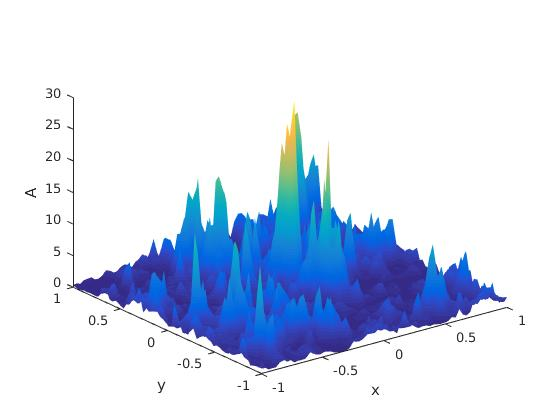
\includegraphics [width=1\linewidth]{Darcy/Pictures/A.jpg}
        \caption{Random field.}
        \label{fig:DarcyA}
    \end{subfigure}
    \begin{subfigure}{0.49\linewidth}
        \centering
        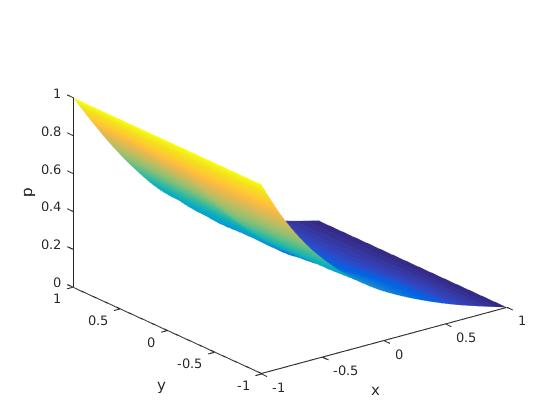
\includegraphics [width=1\linewidth]{Darcy/Pictures/P.jpg}
        \caption{Pressure field.}
        \label{fig:DarcyP}
    \end{subfigure}    
    \begin{subfigure}{0.49\linewidth}
        \centering
        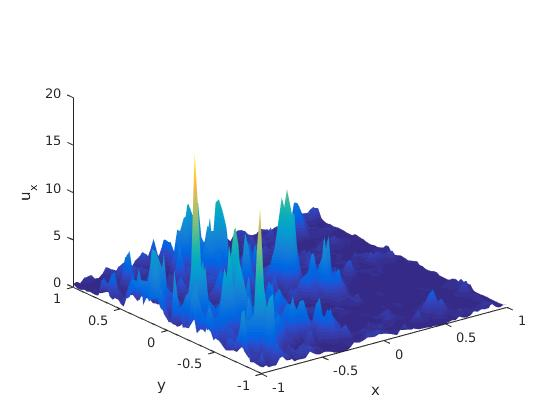
\includegraphics [width=1\linewidth]{Darcy/Pictures/Ux.jpg}
        \caption{$x$ component of velocity field.}
        \label{fig:DarcyUx}
    \end{subfigure}
    \begin{subfigure}{0.49\linewidth}
        \centering
        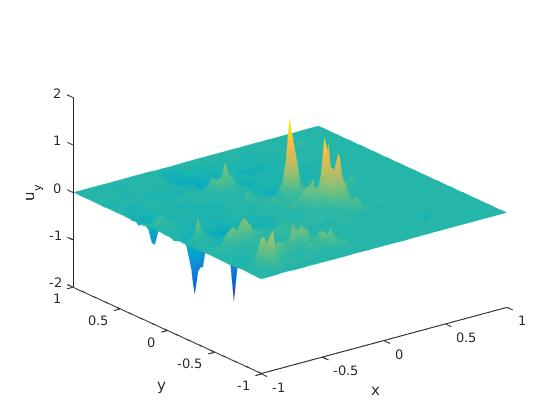
\includegraphics [width=1\linewidth]{Darcy/Pictures/Uy.jpg}
        \caption{$y$ component of velocity field.}
        \label{fig:DarcyUy}
    \end{subfigure}    
    \caption{Approximate solution of the uncertain Darcy problem.}
    \label{fig:DarcyResults}
\end{figure}



\subsection{Finite Elements solution of the Darcy problem}

Let us consider the domain $D = [-1,1] \times [-1,1]$. The random field $A$ in \eqref{eq:DarcyProblem} is chosen to be lognormal, \textit{i.e.}, 
\begin{equation}\label{eq:RandomField}
	A = e^\gamma,
\end{equation}
where $\gamma$ is a normal random field defined by its covariance function $\mathrm{cov}_\gamma(x_1,x_2)$ for any couple of points $x_1,x_2$ in the domain $D$. The covariance function is of the Matern family, thus having the following form
\begin{equation}\label{eq:CovFunction}
	\mathrm{cov}_\gamma(x_1,x_2) = \frac{\sigma^2}{\Gamma(\nu)2^{\nu-1}}\Big(\sqrt{2\nu}\frac{|x_1-x_2|}{L_c}\Big)^\nu K_{\nu}\Big(\sqrt{2\nu}\frac{|x_1-x_2|}{L_c}\Big), \quad \nu \geq 0.5,
\end{equation}
where $\sigma^2$ is the variance, $L_c$ is the correlation length, $\Gamma$ is the gamma function, $K_\nu$ is the modified Bessel function of the second kind and $\nu$ is a parameter. Let us remark that the covariance function does not depend on $x_1, x_2$ but only on their euclidean distance $|x_1 - x_2|$. The regularity of the covariance function and of the realizations of $A$ depend on $\nu$. In particular, for $\nu$ equal to 0.5, the covariance is Lipschitz continuous and the field is $\alpha$-Hölder continuous for $\alpha < 0.5$. Results concerning regularity properties of $A$ can be found in \cite{Nobile2015}. The realizations of $A$ are computed using a discrete Fourier transformation on the vertices of a grid of $D$, equispaced on both the $x$ and $y$ directions with the same spacing $\Delta_A$. Then, the numerical solution $p_h$ of \eqref{eq:DarcyProblem} is obtained with linear Finite Elements on a regular mesh $T_p$ with maximum element size $\Delta_p$. Since the vertices of the grid on which we compute $A$ do not coincide with the vertices of $T_p$, we interpolate $A$ on $T_p$ to obtain $p_h$. Then, the velocity field $u_h$ is retrived computing the gradient on $p_h$. The results for a realization of $A$ are shown in Figure \ref{fig:DarcyResults}, where the value of the inlet pressure $p_0$ is equal to 1, and the parameters for the random field are $\nu = 0.5, L_c = 0.05$. 


\subsection{Solution of the SDE}

Once the Finite Element approximation $u_h$ of the velocity field is available, it is possible to approximate by means of DEM and CEM the solution of \eqref{eq:GeneralDarcySDE}. The values of the numerical solution $X_h$ can take any value in $D$, therefore it is necessary that the velocity field is defined in any point in $D$. If an interpolation of $u_h$ is performed at each step, both DEM and CEM lose in computational efficiency. Hence, an interpolation of $u_h$ has to be performed before the numerical integration of the SDE. We choose to exploit the grid defined by $\Delta_A$, interpolating the values of $u_h$ in the center of each square (Figure \ref{fig:GridVelocity}). Let us denote by $Q$ the set of the interpolation points, whose elements are defined by
\begin{equation}\label{eq:InterpMatrix}
	\{Q\}_{ij} = \begin{pmatrix} -1 + (i-0.5)\Delta_A, & -1 + (j-0.5)\Delta_A \end{pmatrix}^T, \quad i,j = 1, \dots, \frac{2}{\Delta_A} =: N_A.
\end{equation}
We compute two matrices $U_x, U_y$ of $\mathbb{R}^{N_A \times N_A}$ containing the values of the two components of $u_h$ interpolated on the points of $Q$. Then, the velocity field is considered to be piecewise constant in each square of the grid defined by $\Delta_A$. Therefore, if we denote by $\tilde{u}$ the transport field for the SDE, at the $i$-th step of the integration $\tilde{u}$ is evaluated as follows
\begin{equation}\label{eq:VelEval}
	\tilde{u}(X_h(t_i)) = \begin{pmatrix}	U_x(\ceil{(X_{h,1}(t_i)+1)/\Delta_A},\ceil{(X_{h,2}(t_i)+1)/\Delta_A}) \\
					U_y(\ceil{(X_{h,1}(t_i)+1)/\Delta_A},\ceil{(X_{h,2}(t_i)+1)/\Delta_A}) \end{pmatrix},
\end{equation}
where $X_{h,1}, X_{h,2}$ denote the first and second components of $X_h$ and $U_x(i,j)$ represents the element $(i,j)$ of the matrix $U_x$ (respectively $U_y$). Then, given the step size $h$, one step of DEM will be defined as
\begin{equation}\label{eq:DEMDarcy}
	X_h(t_{i+1}) = \tilde{u}(X_h(t_i)) h + \sigma (W(t_{i+1}) - W(t_i)).
\end{equation}

\begin{figure}[t]
    \centering
    \resizebox{0.8\linewidth}{!}{% This file was created by matlab2tikz.
%
%The latest updates can be retrieved from
%  http://www.mathworks.com/matlabcentral/fileexchange/22022-matlab2tikz-matlab2tikz
%where you can also make suggestions and rate matlab2tikz.
%
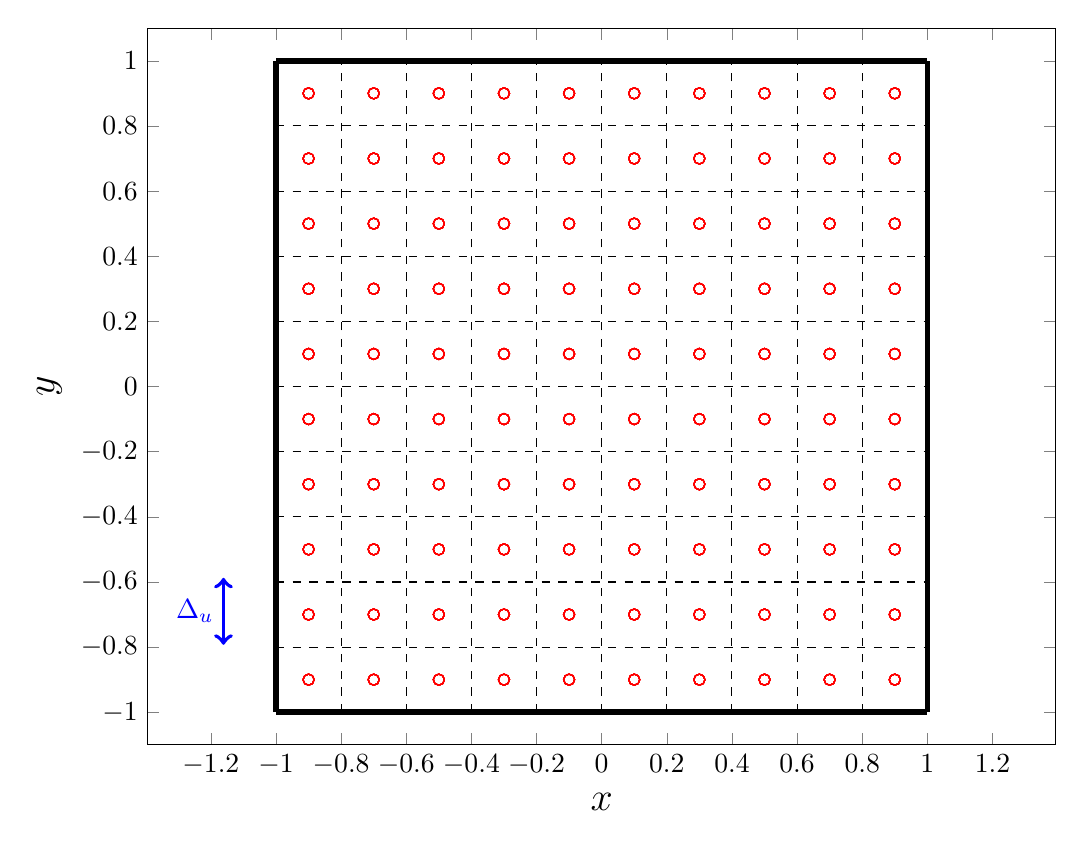
\begin{tikzpicture}



\begin{axis}[%
width=4.542in,
height=3.583in,
at={(0.801in,0.484in)},
scale only axis,
xmin=-1.39468302658487,
xmax=1.39468302658487,
xlabel={$x$},
xlabel style={font=\Large},
ymin=-1.1,
ymax=1.1,
ylabel={$y$},
ylabel style={font=\Large},
axis background/.style={fill=white}
]
\addplot [color=black,solid,line width=2.0pt,forget plot]
  table[row sep=crcr]{%
-1	-1\\
-1	1\\
};
\addplot [color=black,solid,line width=2.0pt,forget plot]
  table[row sep=crcr]{%
1	-1\\
1	1\\
};
\addplot [color=black,solid,line width=2.0pt,forget plot]
  table[row sep=crcr]{%
-1	-1\\
1	-1\\
};
\addplot [color=black,solid,line width=2.0pt,forget plot]
  table[row sep=crcr]{%
-1	1\\
1	1\\
};
\addplot [color=black,dashed,forget plot]
  table[row sep=crcr]{%
-1	-0.8\\
1	-0.8\\
};
\addplot [color=black,dashed,forget plot]
  table[row sep=crcr]{%
-0.8	-1\\
-0.8	1\\
};
\addplot [color=red,only marks,mark=o,mark options={solid},forget plot]
  table[row sep=crcr]{%
-0.9	-0.9\\
-0.9	-0.7\\
-0.9	-0.5\\
-0.9	-0.3\\
-0.9	-0.1\\
-0.9	0.1\\
-0.9	0.3\\
-0.9	0.5\\
-0.9	0.7\\
-0.9	0.9\\
};
\addplot [color=red,only marks,mark=o,mark options={solid},forget plot]
  table[row sep=crcr]{%
-0.9	-0.9\\
-0.9	-0.7\\
-0.9	-0.5\\
-0.9	-0.3\\
-0.9	-0.1\\
-0.9	0.1\\
-0.9	0.3\\
-0.9	0.5\\
-0.9	0.7\\
-0.9	0.9\\
};
\addplot [color=red,only marks,mark=o,mark options={solid},forget plot]
  table[row sep=crcr]{%
-0.9	-0.9\\
-0.9	-0.7\\
-0.9	-0.5\\
-0.9	-0.3\\
-0.9	-0.1\\
-0.9	0.1\\
-0.9	0.3\\
-0.9	0.5\\
-0.9	0.7\\
-0.9	0.9\\
};
\addplot [color=red,only marks,mark=o,mark options={solid},forget plot]
  table[row sep=crcr]{%
-0.9	-0.9\\
-0.9	-0.7\\
-0.9	-0.5\\
-0.9	-0.3\\
-0.9	-0.1\\
-0.9	0.1\\
-0.9	0.3\\
-0.9	0.5\\
-0.9	0.7\\
-0.9	0.9\\
};
\addplot [color=red,only marks,mark=o,mark options={solid},forget plot]
  table[row sep=crcr]{%
-0.9	-0.9\\
-0.9	-0.7\\
-0.9	-0.5\\
-0.9	-0.3\\
-0.9	-0.1\\
-0.9	0.1\\
-0.9	0.3\\
-0.9	0.5\\
-0.9	0.7\\
-0.9	0.9\\
};
\addplot [color=red,only marks,mark=o,mark options={solid},forget plot]
  table[row sep=crcr]{%
-0.9	-0.9\\
-0.9	-0.7\\
-0.9	-0.5\\
-0.9	-0.3\\
-0.9	-0.1\\
-0.9	0.1\\
-0.9	0.3\\
-0.9	0.5\\
-0.9	0.7\\
-0.9	0.9\\
};
\addplot [color=red,only marks,mark=o,mark options={solid},forget plot]
  table[row sep=crcr]{%
-0.9	-0.9\\
-0.9	-0.7\\
-0.9	-0.5\\
-0.9	-0.3\\
-0.9	-0.1\\
-0.9	0.1\\
-0.9	0.3\\
-0.9	0.5\\
-0.9	0.7\\
-0.9	0.9\\
};
\addplot [color=red,only marks,mark=o,mark options={solid},forget plot]
  table[row sep=crcr]{%
-0.9	-0.9\\
-0.9	-0.7\\
-0.9	-0.5\\
-0.9	-0.3\\
-0.9	-0.1\\
-0.9	0.1\\
-0.9	0.3\\
-0.9	0.5\\
-0.9	0.7\\
-0.9	0.9\\
};
\addplot [color=red,only marks,mark=o,mark options={solid},forget plot]
  table[row sep=crcr]{%
-0.9	-0.9\\
-0.9	-0.7\\
-0.9	-0.5\\
-0.9	-0.3\\
-0.9	-0.1\\
-0.9	0.1\\
-0.9	0.3\\
-0.9	0.5\\
-0.9	0.7\\
-0.9	0.9\\
};
\addplot [color=red,only marks,mark=o,mark options={solid},forget plot]
  table[row sep=crcr]{%
-0.9	-0.9\\
-0.9	-0.7\\
-0.9	-0.5\\
-0.9	-0.3\\
-0.9	-0.1\\
-0.9	0.1\\
-0.9	0.3\\
-0.9	0.5\\
-0.9	0.7\\
-0.9	0.9\\
};
\addplot [color=black,dashed,forget plot]
  table[row sep=crcr]{%
-1	-0.6\\
1	-0.6\\
};
\addplot [color=black,dashed,forget plot]
  table[row sep=crcr]{%
-0.6	-1\\
-0.6	1\\
};
\addplot [color=red,only marks,mark=o,mark options={solid},forget plot]
  table[row sep=crcr]{%
-0.7	-0.9\\
-0.7	-0.7\\
-0.7	-0.5\\
-0.7	-0.3\\
-0.7	-0.1\\
-0.7	0.1\\
-0.7	0.3\\
-0.7	0.5\\
-0.7	0.7\\
-0.7	0.9\\
};
\addplot [color=red,only marks,mark=o,mark options={solid},forget plot]
  table[row sep=crcr]{%
-0.7	-0.9\\
-0.7	-0.7\\
-0.7	-0.5\\
-0.7	-0.3\\
-0.7	-0.1\\
-0.7	0.1\\
-0.7	0.3\\
-0.7	0.5\\
-0.7	0.7\\
-0.7	0.9\\
};
\addplot [color=red,only marks,mark=o,mark options={solid},forget plot]
  table[row sep=crcr]{%
-0.7	-0.9\\
-0.7	-0.7\\
-0.7	-0.5\\
-0.7	-0.3\\
-0.7	-0.1\\
-0.7	0.1\\
-0.7	0.3\\
-0.7	0.5\\
-0.7	0.7\\
-0.7	0.9\\
};
\addplot [color=red,only marks,mark=o,mark options={solid},forget plot]
  table[row sep=crcr]{%
-0.7	-0.9\\
-0.7	-0.7\\
-0.7	-0.5\\
-0.7	-0.3\\
-0.7	-0.1\\
-0.7	0.1\\
-0.7	0.3\\
-0.7	0.5\\
-0.7	0.7\\
-0.7	0.9\\
};
\addplot [color=red,only marks,mark=o,mark options={solid},forget plot]
  table[row sep=crcr]{%
-0.7	-0.9\\
-0.7	-0.7\\
-0.7	-0.5\\
-0.7	-0.3\\
-0.7	-0.1\\
-0.7	0.1\\
-0.7	0.3\\
-0.7	0.5\\
-0.7	0.7\\
-0.7	0.9\\
};
\addplot [color=red,only marks,mark=o,mark options={solid},forget plot]
  table[row sep=crcr]{%
-0.7	-0.9\\
-0.7	-0.7\\
-0.7	-0.5\\
-0.7	-0.3\\
-0.7	-0.1\\
-0.7	0.1\\
-0.7	0.3\\
-0.7	0.5\\
-0.7	0.7\\
-0.7	0.9\\
};
\addplot [color=red,only marks,mark=o,mark options={solid},forget plot]
  table[row sep=crcr]{%
-0.7	-0.9\\
-0.7	-0.7\\
-0.7	-0.5\\
-0.7	-0.3\\
-0.7	-0.1\\
-0.7	0.1\\
-0.7	0.3\\
-0.7	0.5\\
-0.7	0.7\\
-0.7	0.9\\
};
\addplot [color=red,only marks,mark=o,mark options={solid},forget plot]
  table[row sep=crcr]{%
-0.7	-0.9\\
-0.7	-0.7\\
-0.7	-0.5\\
-0.7	-0.3\\
-0.7	-0.1\\
-0.7	0.1\\
-0.7	0.3\\
-0.7	0.5\\
-0.7	0.7\\
-0.7	0.9\\
};
\addplot [color=red,only marks,mark=o,mark options={solid},forget plot]
  table[row sep=crcr]{%
-0.7	-0.9\\
-0.7	-0.7\\
-0.7	-0.5\\
-0.7	-0.3\\
-0.7	-0.1\\
-0.7	0.1\\
-0.7	0.3\\
-0.7	0.5\\
-0.7	0.7\\
-0.7	0.9\\
};
\addplot [color=red,only marks,mark=o,mark options={solid},forget plot]
  table[row sep=crcr]{%
-0.7	-0.9\\
-0.7	-0.7\\
-0.7	-0.5\\
-0.7	-0.3\\
-0.7	-0.1\\
-0.7	0.1\\
-0.7	0.3\\
-0.7	0.5\\
-0.7	0.7\\
-0.7	0.9\\
};
\addplot [color=black,dashed,forget plot]
  table[row sep=crcr]{%
-1	-0.4\\
1	-0.4\\
};
\addplot [color=black,dashed,forget plot]
  table[row sep=crcr]{%
-0.4	-1\\
-0.4	1\\
};
\addplot [color=red,only marks,mark=o,mark options={solid},forget plot]
  table[row sep=crcr]{%
-0.5	-0.9\\
-0.5	-0.7\\
-0.5	-0.5\\
-0.5	-0.3\\
-0.5	-0.1\\
-0.5	0.1\\
-0.5	0.3\\
-0.5	0.5\\
-0.5	0.7\\
-0.5	0.9\\
};
\addplot [color=red,only marks,mark=o,mark options={solid},forget plot]
  table[row sep=crcr]{%
-0.5	-0.9\\
-0.5	-0.7\\
-0.5	-0.5\\
-0.5	-0.3\\
-0.5	-0.1\\
-0.5	0.1\\
-0.5	0.3\\
-0.5	0.5\\
-0.5	0.7\\
-0.5	0.9\\
};
\addplot [color=red,only marks,mark=o,mark options={solid},forget plot]
  table[row sep=crcr]{%
-0.5	-0.9\\
-0.5	-0.7\\
-0.5	-0.5\\
-0.5	-0.3\\
-0.5	-0.1\\
-0.5	0.1\\
-0.5	0.3\\
-0.5	0.5\\
-0.5	0.7\\
-0.5	0.9\\
};
\addplot [color=red,only marks,mark=o,mark options={solid},forget plot]
  table[row sep=crcr]{%
-0.5	-0.9\\
-0.5	-0.7\\
-0.5	-0.5\\
-0.5	-0.3\\
-0.5	-0.1\\
-0.5	0.1\\
-0.5	0.3\\
-0.5	0.5\\
-0.5	0.7\\
-0.5	0.9\\
};
\addplot [color=red,only marks,mark=o,mark options={solid},forget plot]
  table[row sep=crcr]{%
-0.5	-0.9\\
-0.5	-0.7\\
-0.5	-0.5\\
-0.5	-0.3\\
-0.5	-0.1\\
-0.5	0.1\\
-0.5	0.3\\
-0.5	0.5\\
-0.5	0.7\\
-0.5	0.9\\
};
\addplot [color=red,only marks,mark=o,mark options={solid},forget plot]
  table[row sep=crcr]{%
-0.5	-0.9\\
-0.5	-0.7\\
-0.5	-0.5\\
-0.5	-0.3\\
-0.5	-0.1\\
-0.5	0.1\\
-0.5	0.3\\
-0.5	0.5\\
-0.5	0.7\\
-0.5	0.9\\
};
\addplot [color=red,only marks,mark=o,mark options={solid},forget plot]
  table[row sep=crcr]{%
-0.5	-0.9\\
-0.5	-0.7\\
-0.5	-0.5\\
-0.5	-0.3\\
-0.5	-0.1\\
-0.5	0.1\\
-0.5	0.3\\
-0.5	0.5\\
-0.5	0.7\\
-0.5	0.9\\
};
\addplot [color=red,only marks,mark=o,mark options={solid},forget plot]
  table[row sep=crcr]{%
-0.5	-0.9\\
-0.5	-0.7\\
-0.5	-0.5\\
-0.5	-0.3\\
-0.5	-0.1\\
-0.5	0.1\\
-0.5	0.3\\
-0.5	0.5\\
-0.5	0.7\\
-0.5	0.9\\
};
\addplot [color=red,only marks,mark=o,mark options={solid},forget plot]
  table[row sep=crcr]{%
-0.5	-0.9\\
-0.5	-0.7\\
-0.5	-0.5\\
-0.5	-0.3\\
-0.5	-0.1\\
-0.5	0.1\\
-0.5	0.3\\
-0.5	0.5\\
-0.5	0.7\\
-0.5	0.9\\
};
\addplot [color=red,only marks,mark=o,mark options={solid},forget plot]
  table[row sep=crcr]{%
-0.5	-0.9\\
-0.5	-0.7\\
-0.5	-0.5\\
-0.5	-0.3\\
-0.5	-0.1\\
-0.5	0.1\\
-0.5	0.3\\
-0.5	0.5\\
-0.5	0.7\\
-0.5	0.9\\
};
\addplot [color=black,dashed,forget plot]
  table[row sep=crcr]{%
-1	-0.2\\
1	-0.2\\
};
\addplot [color=black,dashed,forget plot]
  table[row sep=crcr]{%
-0.2	-1\\
-0.2	1\\
};
\addplot [color=red,only marks,mark=o,mark options={solid},forget plot]
  table[row sep=crcr]{%
-0.3	-0.9\\
-0.3	-0.7\\
-0.3	-0.5\\
-0.3	-0.3\\
-0.3	-0.1\\
-0.3	0.1\\
-0.3	0.3\\
-0.3	0.5\\
-0.3	0.7\\
-0.3	0.9\\
};
\addplot [color=red,only marks,mark=o,mark options={solid},forget plot]
  table[row sep=crcr]{%
-0.3	-0.9\\
-0.3	-0.7\\
-0.3	-0.5\\
-0.3	-0.3\\
-0.3	-0.1\\
-0.3	0.1\\
-0.3	0.3\\
-0.3	0.5\\
-0.3	0.7\\
-0.3	0.9\\
};
\addplot [color=red,only marks,mark=o,mark options={solid},forget plot]
  table[row sep=crcr]{%
-0.3	-0.9\\
-0.3	-0.7\\
-0.3	-0.5\\
-0.3	-0.3\\
-0.3	-0.1\\
-0.3	0.1\\
-0.3	0.3\\
-0.3	0.5\\
-0.3	0.7\\
-0.3	0.9\\
};
\addplot [color=red,only marks,mark=o,mark options={solid},forget plot]
  table[row sep=crcr]{%
-0.3	-0.9\\
-0.3	-0.7\\
-0.3	-0.5\\
-0.3	-0.3\\
-0.3	-0.1\\
-0.3	0.1\\
-0.3	0.3\\
-0.3	0.5\\
-0.3	0.7\\
-0.3	0.9\\
};
\addplot [color=red,only marks,mark=o,mark options={solid},forget plot]
  table[row sep=crcr]{%
-0.3	-0.9\\
-0.3	-0.7\\
-0.3	-0.5\\
-0.3	-0.3\\
-0.3	-0.1\\
-0.3	0.1\\
-0.3	0.3\\
-0.3	0.5\\
-0.3	0.7\\
-0.3	0.9\\
};
\addplot [color=red,only marks,mark=o,mark options={solid},forget plot]
  table[row sep=crcr]{%
-0.3	-0.9\\
-0.3	-0.7\\
-0.3	-0.5\\
-0.3	-0.3\\
-0.3	-0.1\\
-0.3	0.1\\
-0.3	0.3\\
-0.3	0.5\\
-0.3	0.7\\
-0.3	0.9\\
};
\addplot [color=red,only marks,mark=o,mark options={solid},forget plot]
  table[row sep=crcr]{%
-0.3	-0.9\\
-0.3	-0.7\\
-0.3	-0.5\\
-0.3	-0.3\\
-0.3	-0.1\\
-0.3	0.1\\
-0.3	0.3\\
-0.3	0.5\\
-0.3	0.7\\
-0.3	0.9\\
};
\addplot [color=red,only marks,mark=o,mark options={solid},forget plot]
  table[row sep=crcr]{%
-0.3	-0.9\\
-0.3	-0.7\\
-0.3	-0.5\\
-0.3	-0.3\\
-0.3	-0.1\\
-0.3	0.1\\
-0.3	0.3\\
-0.3	0.5\\
-0.3	0.7\\
-0.3	0.9\\
};
\addplot [color=red,only marks,mark=o,mark options={solid},forget plot]
  table[row sep=crcr]{%
-0.3	-0.9\\
-0.3	-0.7\\
-0.3	-0.5\\
-0.3	-0.3\\
-0.3	-0.1\\
-0.3	0.1\\
-0.3	0.3\\
-0.3	0.5\\
-0.3	0.7\\
-0.3	0.9\\
};
\addplot [color=red,only marks,mark=o,mark options={solid},forget plot]
  table[row sep=crcr]{%
-0.3	-0.9\\
-0.3	-0.7\\
-0.3	-0.5\\
-0.3	-0.3\\
-0.3	-0.1\\
-0.3	0.1\\
-0.3	0.3\\
-0.3	0.5\\
-0.3	0.7\\
-0.3	0.9\\
};
\addplot [color=black,dashed,forget plot]
  table[row sep=crcr]{%
-1	0\\
1	0\\
};
\addplot [color=black,dashed,forget plot]
  table[row sep=crcr]{%
0	-1\\
0	1\\
};
\addplot [color=red,only marks,mark=o,mark options={solid},forget plot]
  table[row sep=crcr]{%
-0.1	-0.9\\
-0.1	-0.7\\
-0.1	-0.5\\
-0.1	-0.3\\
-0.1	-0.1\\
-0.1	0.1\\
-0.1	0.3\\
-0.1	0.5\\
-0.1	0.7\\
-0.1	0.9\\
};
\addplot [color=red,only marks,mark=o,mark options={solid},forget plot]
  table[row sep=crcr]{%
-0.1	-0.9\\
-0.1	-0.7\\
-0.1	-0.5\\
-0.1	-0.3\\
-0.1	-0.1\\
-0.1	0.1\\
-0.1	0.3\\
-0.1	0.5\\
-0.1	0.7\\
-0.1	0.9\\
};
\addplot [color=red,only marks,mark=o,mark options={solid},forget plot]
  table[row sep=crcr]{%
-0.1	-0.9\\
-0.1	-0.7\\
-0.1	-0.5\\
-0.1	-0.3\\
-0.1	-0.1\\
-0.1	0.1\\
-0.1	0.3\\
-0.1	0.5\\
-0.1	0.7\\
-0.1	0.9\\
};
\addplot [color=red,only marks,mark=o,mark options={solid},forget plot]
  table[row sep=crcr]{%
-0.1	-0.9\\
-0.1	-0.7\\
-0.1	-0.5\\
-0.1	-0.3\\
-0.1	-0.1\\
-0.1	0.1\\
-0.1	0.3\\
-0.1	0.5\\
-0.1	0.7\\
-0.1	0.9\\
};
\addplot [color=red,only marks,mark=o,mark options={solid},forget plot]
  table[row sep=crcr]{%
-0.1	-0.9\\
-0.1	-0.7\\
-0.1	-0.5\\
-0.1	-0.3\\
-0.1	-0.1\\
-0.1	0.1\\
-0.1	0.3\\
-0.1	0.5\\
-0.1	0.7\\
-0.1	0.9\\
};
\addplot [color=red,only marks,mark=o,mark options={solid},forget plot]
  table[row sep=crcr]{%
-0.1	-0.9\\
-0.1	-0.7\\
-0.1	-0.5\\
-0.1	-0.3\\
-0.1	-0.1\\
-0.1	0.1\\
-0.1	0.3\\
-0.1	0.5\\
-0.1	0.7\\
-0.1	0.9\\
};
\addplot [color=red,only marks,mark=o,mark options={solid},forget plot]
  table[row sep=crcr]{%
-0.1	-0.9\\
-0.1	-0.7\\
-0.1	-0.5\\
-0.1	-0.3\\
-0.1	-0.1\\
-0.1	0.1\\
-0.1	0.3\\
-0.1	0.5\\
-0.1	0.7\\
-0.1	0.9\\
};
\addplot [color=red,only marks,mark=o,mark options={solid},forget plot]
  table[row sep=crcr]{%
-0.1	-0.9\\
-0.1	-0.7\\
-0.1	-0.5\\
-0.1	-0.3\\
-0.1	-0.1\\
-0.1	0.1\\
-0.1	0.3\\
-0.1	0.5\\
-0.1	0.7\\
-0.1	0.9\\
};
\addplot [color=red,only marks,mark=o,mark options={solid},forget plot]
  table[row sep=crcr]{%
-0.1	-0.9\\
-0.1	-0.7\\
-0.1	-0.5\\
-0.1	-0.3\\
-0.1	-0.1\\
-0.1	0.1\\
-0.1	0.3\\
-0.1	0.5\\
-0.1	0.7\\
-0.1	0.9\\
};
\addplot [color=red,only marks,mark=o,mark options={solid},forget plot]
  table[row sep=crcr]{%
-0.1	-0.9\\
-0.1	-0.7\\
-0.1	-0.5\\
-0.1	-0.3\\
-0.1	-0.1\\
-0.1	0.1\\
-0.1	0.3\\
-0.1	0.5\\
-0.1	0.7\\
-0.1	0.9\\
};
\addplot [color=black,dashed,forget plot]
  table[row sep=crcr]{%
-1	0.2\\
1	0.2\\
};
\addplot [color=black,dashed,forget plot]
  table[row sep=crcr]{%
0.2	-1\\
0.2	1\\
};
\addplot [color=red,only marks,mark=o,mark options={solid},forget plot]
  table[row sep=crcr]{%
0.1	-0.9\\
0.1	-0.7\\
0.1	-0.5\\
0.1	-0.3\\
0.1	-0.1\\
0.1	0.1\\
0.1	0.3\\
0.1	0.5\\
0.1	0.7\\
0.1	0.9\\
};
\addplot [color=red,only marks,mark=o,mark options={solid},forget plot]
  table[row sep=crcr]{%
0.1	-0.9\\
0.1	-0.7\\
0.1	-0.5\\
0.1	-0.3\\
0.1	-0.1\\
0.1	0.1\\
0.1	0.3\\
0.1	0.5\\
0.1	0.7\\
0.1	0.9\\
};
\addplot [color=red,only marks,mark=o,mark options={solid},forget plot]
  table[row sep=crcr]{%
0.1	-0.9\\
0.1	-0.7\\
0.1	-0.5\\
0.1	-0.3\\
0.1	-0.1\\
0.1	0.1\\
0.1	0.3\\
0.1	0.5\\
0.1	0.7\\
0.1	0.9\\
};
\addplot [color=red,only marks,mark=o,mark options={solid},forget plot]
  table[row sep=crcr]{%
0.1	-0.9\\
0.1	-0.7\\
0.1	-0.5\\
0.1	-0.3\\
0.1	-0.1\\
0.1	0.1\\
0.1	0.3\\
0.1	0.5\\
0.1	0.7\\
0.1	0.9\\
};
\addplot [color=red,only marks,mark=o,mark options={solid},forget plot]
  table[row sep=crcr]{%
0.1	-0.9\\
0.1	-0.7\\
0.1	-0.5\\
0.1	-0.3\\
0.1	-0.1\\
0.1	0.1\\
0.1	0.3\\
0.1	0.5\\
0.1	0.7\\
0.1	0.9\\
};
\addplot [color=red,only marks,mark=o,mark options={solid},forget plot]
  table[row sep=crcr]{%
0.1	-0.9\\
0.1	-0.7\\
0.1	-0.5\\
0.1	-0.3\\
0.1	-0.1\\
0.1	0.1\\
0.1	0.3\\
0.1	0.5\\
0.1	0.7\\
0.1	0.9\\
};
\addplot [color=red,only marks,mark=o,mark options={solid},forget plot]
  table[row sep=crcr]{%
0.1	-0.9\\
0.1	-0.7\\
0.1	-0.5\\
0.1	-0.3\\
0.1	-0.1\\
0.1	0.1\\
0.1	0.3\\
0.1	0.5\\
0.1	0.7\\
0.1	0.9\\
};
\addplot [color=red,only marks,mark=o,mark options={solid},forget plot]
  table[row sep=crcr]{%
0.1	-0.9\\
0.1	-0.7\\
0.1	-0.5\\
0.1	-0.3\\
0.1	-0.1\\
0.1	0.1\\
0.1	0.3\\
0.1	0.5\\
0.1	0.7\\
0.1	0.9\\
};
\addplot [color=red,only marks,mark=o,mark options={solid},forget plot]
  table[row sep=crcr]{%
0.1	-0.9\\
0.1	-0.7\\
0.1	-0.5\\
0.1	-0.3\\
0.1	-0.1\\
0.1	0.1\\
0.1	0.3\\
0.1	0.5\\
0.1	0.7\\
0.1	0.9\\
};
\addplot [color=red,only marks,mark=o,mark options={solid},forget plot]
  table[row sep=crcr]{%
0.1	-0.9\\
0.1	-0.7\\
0.1	-0.5\\
0.1	-0.3\\
0.1	-0.1\\
0.1	0.1\\
0.1	0.3\\
0.1	0.5\\
0.1	0.7\\
0.1	0.9\\
};
\addplot [color=black,dashed,forget plot]
  table[row sep=crcr]{%
-1	0.4\\
1	0.4\\
};
\addplot [color=black,dashed,forget plot]
  table[row sep=crcr]{%
0.4	-1\\
0.4	1\\
};
\addplot [color=red,only marks,mark=o,mark options={solid},forget plot]
  table[row sep=crcr]{%
0.3	-0.9\\
0.3	-0.7\\
0.3	-0.5\\
0.3	-0.3\\
0.3	-0.1\\
0.3	0.1\\
0.3	0.3\\
0.3	0.5\\
0.3	0.7\\
0.3	0.9\\
};
\addplot [color=red,only marks,mark=o,mark options={solid},forget plot]
  table[row sep=crcr]{%
0.3	-0.9\\
0.3	-0.7\\
0.3	-0.5\\
0.3	-0.3\\
0.3	-0.1\\
0.3	0.1\\
0.3	0.3\\
0.3	0.5\\
0.3	0.7\\
0.3	0.9\\
};
\addplot [color=red,only marks,mark=o,mark options={solid},forget plot]
  table[row sep=crcr]{%
0.3	-0.9\\
0.3	-0.7\\
0.3	-0.5\\
0.3	-0.3\\
0.3	-0.1\\
0.3	0.1\\
0.3	0.3\\
0.3	0.5\\
0.3	0.7\\
0.3	0.9\\
};
\addplot [color=red,only marks,mark=o,mark options={solid},forget plot]
  table[row sep=crcr]{%
0.3	-0.9\\
0.3	-0.7\\
0.3	-0.5\\
0.3	-0.3\\
0.3	-0.1\\
0.3	0.1\\
0.3	0.3\\
0.3	0.5\\
0.3	0.7\\
0.3	0.9\\
};
\addplot [color=red,only marks,mark=o,mark options={solid},forget plot]
  table[row sep=crcr]{%
0.3	-0.9\\
0.3	-0.7\\
0.3	-0.5\\
0.3	-0.3\\
0.3	-0.1\\
0.3	0.1\\
0.3	0.3\\
0.3	0.5\\
0.3	0.7\\
0.3	0.9\\
};
\addplot [color=red,only marks,mark=o,mark options={solid},forget plot]
  table[row sep=crcr]{%
0.3	-0.9\\
0.3	-0.7\\
0.3	-0.5\\
0.3	-0.3\\
0.3	-0.1\\
0.3	0.1\\
0.3	0.3\\
0.3	0.5\\
0.3	0.7\\
0.3	0.9\\
};
\addplot [color=red,only marks,mark=o,mark options={solid},forget plot]
  table[row sep=crcr]{%
0.3	-0.9\\
0.3	-0.7\\
0.3	-0.5\\
0.3	-0.3\\
0.3	-0.1\\
0.3	0.1\\
0.3	0.3\\
0.3	0.5\\
0.3	0.7\\
0.3	0.9\\
};
\addplot [color=red,only marks,mark=o,mark options={solid},forget plot]
  table[row sep=crcr]{%
0.3	-0.9\\
0.3	-0.7\\
0.3	-0.5\\
0.3	-0.3\\
0.3	-0.1\\
0.3	0.1\\
0.3	0.3\\
0.3	0.5\\
0.3	0.7\\
0.3	0.9\\
};
\addplot [color=red,only marks,mark=o,mark options={solid},forget plot]
  table[row sep=crcr]{%
0.3	-0.9\\
0.3	-0.7\\
0.3	-0.5\\
0.3	-0.3\\
0.3	-0.1\\
0.3	0.1\\
0.3	0.3\\
0.3	0.5\\
0.3	0.7\\
0.3	0.9\\
};
\addplot [color=red,only marks,mark=o,mark options={solid},forget plot]
  table[row sep=crcr]{%
0.3	-0.9\\
0.3	-0.7\\
0.3	-0.5\\
0.3	-0.3\\
0.3	-0.1\\
0.3	0.1\\
0.3	0.3\\
0.3	0.5\\
0.3	0.7\\
0.3	0.9\\
};
\addplot [color=black,dashed,forget plot]
  table[row sep=crcr]{%
-1	0.6\\
1	0.6\\
};
\addplot [color=black,dashed,forget plot]
  table[row sep=crcr]{%
0.6	-1\\
0.6	1\\
};
\addplot [color=red,only marks,mark=o,mark options={solid},forget plot]
  table[row sep=crcr]{%
0.5	-0.9\\
0.5	-0.7\\
0.5	-0.5\\
0.5	-0.3\\
0.5	-0.1\\
0.5	0.1\\
0.5	0.3\\
0.5	0.5\\
0.5	0.7\\
0.5	0.9\\
};
\addplot [color=red,only marks,mark=o,mark options={solid},forget plot]
  table[row sep=crcr]{%
0.5	-0.9\\
0.5	-0.7\\
0.5	-0.5\\
0.5	-0.3\\
0.5	-0.1\\
0.5	0.1\\
0.5	0.3\\
0.5	0.5\\
0.5	0.7\\
0.5	0.9\\
};
\addplot [color=red,only marks,mark=o,mark options={solid},forget plot]
  table[row sep=crcr]{%
0.5	-0.9\\
0.5	-0.7\\
0.5	-0.5\\
0.5	-0.3\\
0.5	-0.1\\
0.5	0.1\\
0.5	0.3\\
0.5	0.5\\
0.5	0.7\\
0.5	0.9\\
};
\addplot [color=red,only marks,mark=o,mark options={solid},forget plot]
  table[row sep=crcr]{%
0.5	-0.9\\
0.5	-0.7\\
0.5	-0.5\\
0.5	-0.3\\
0.5	-0.1\\
0.5	0.1\\
0.5	0.3\\
0.5	0.5\\
0.5	0.7\\
0.5	0.9\\
};
\addplot [color=red,only marks,mark=o,mark options={solid},forget plot]
  table[row sep=crcr]{%
0.5	-0.9\\
0.5	-0.7\\
0.5	-0.5\\
0.5	-0.3\\
0.5	-0.1\\
0.5	0.1\\
0.5	0.3\\
0.5	0.5\\
0.5	0.7\\
0.5	0.9\\
};
\addplot [color=red,only marks,mark=o,mark options={solid},forget plot]
  table[row sep=crcr]{%
0.5	-0.9\\
0.5	-0.7\\
0.5	-0.5\\
0.5	-0.3\\
0.5	-0.1\\
0.5	0.1\\
0.5	0.3\\
0.5	0.5\\
0.5	0.7\\
0.5	0.9\\
};
\addplot [color=red,only marks,mark=o,mark options={solid},forget plot]
  table[row sep=crcr]{%
0.5	-0.9\\
0.5	-0.7\\
0.5	-0.5\\
0.5	-0.3\\
0.5	-0.1\\
0.5	0.1\\
0.5	0.3\\
0.5	0.5\\
0.5	0.7\\
0.5	0.9\\
};
\addplot [color=red,only marks,mark=o,mark options={solid},forget plot]
  table[row sep=crcr]{%
0.5	-0.9\\
0.5	-0.7\\
0.5	-0.5\\
0.5	-0.3\\
0.5	-0.1\\
0.5	0.1\\
0.5	0.3\\
0.5	0.5\\
0.5	0.7\\
0.5	0.9\\
};
\addplot [color=red,only marks,mark=o,mark options={solid},forget plot]
  table[row sep=crcr]{%
0.5	-0.9\\
0.5	-0.7\\
0.5	-0.5\\
0.5	-0.3\\
0.5	-0.1\\
0.5	0.1\\
0.5	0.3\\
0.5	0.5\\
0.5	0.7\\
0.5	0.9\\
};
\addplot [color=red,only marks,mark=o,mark options={solid},forget plot]
  table[row sep=crcr]{%
0.5	-0.9\\
0.5	-0.7\\
0.5	-0.5\\
0.5	-0.3\\
0.5	-0.1\\
0.5	0.1\\
0.5	0.3\\
0.5	0.5\\
0.5	0.7\\
0.5	0.9\\
};
\addplot [color=black,dashed,forget plot]
  table[row sep=crcr]{%
-1	0.8\\
1	0.8\\
};
\addplot [color=black,dashed,forget plot]
  table[row sep=crcr]{%
0.8	-1\\
0.8	1\\
};
\addplot [color=red,only marks,mark=o,mark options={solid},forget plot]
  table[row sep=crcr]{%
0.7	-0.9\\
0.7	-0.7\\
0.7	-0.5\\
0.7	-0.3\\
0.7	-0.1\\
0.7	0.1\\
0.7	0.3\\
0.7	0.5\\
0.7	0.7\\
0.7	0.9\\
};
\addplot [color=red,only marks,mark=o,mark options={solid},forget plot]
  table[row sep=crcr]{%
0.7	-0.9\\
0.7	-0.7\\
0.7	-0.5\\
0.7	-0.3\\
0.7	-0.1\\
0.7	0.1\\
0.7	0.3\\
0.7	0.5\\
0.7	0.7\\
0.7	0.9\\
};
\addplot [color=red,only marks,mark=o,mark options={solid},forget plot]
  table[row sep=crcr]{%
0.7	-0.9\\
0.7	-0.7\\
0.7	-0.5\\
0.7	-0.3\\
0.7	-0.1\\
0.7	0.1\\
0.7	0.3\\
0.7	0.5\\
0.7	0.7\\
0.7	0.9\\
};
\addplot [color=red,only marks,mark=o,mark options={solid},forget plot]
  table[row sep=crcr]{%
0.7	-0.9\\
0.7	-0.7\\
0.7	-0.5\\
0.7	-0.3\\
0.7	-0.1\\
0.7	0.1\\
0.7	0.3\\
0.7	0.5\\
0.7	0.7\\
0.7	0.9\\
};
\addplot [color=red,only marks,mark=o,mark options={solid},forget plot]
  table[row sep=crcr]{%
0.7	-0.9\\
0.7	-0.7\\
0.7	-0.5\\
0.7	-0.3\\
0.7	-0.1\\
0.7	0.1\\
0.7	0.3\\
0.7	0.5\\
0.7	0.7\\
0.7	0.9\\
};
\addplot [color=red,only marks,mark=o,mark options={solid},forget plot]
  table[row sep=crcr]{%
0.7	-0.9\\
0.7	-0.7\\
0.7	-0.5\\
0.7	-0.3\\
0.7	-0.1\\
0.7	0.1\\
0.7	0.3\\
0.7	0.5\\
0.7	0.7\\
0.7	0.9\\
};
\addplot [color=red,only marks,mark=o,mark options={solid},forget plot]
  table[row sep=crcr]{%
0.7	-0.9\\
0.7	-0.7\\
0.7	-0.5\\
0.7	-0.3\\
0.7	-0.1\\
0.7	0.1\\
0.7	0.3\\
0.7	0.5\\
0.7	0.7\\
0.7	0.9\\
};
\addplot [color=red,only marks,mark=o,mark options={solid},forget plot]
  table[row sep=crcr]{%
0.7	-0.9\\
0.7	-0.7\\
0.7	-0.5\\
0.7	-0.3\\
0.7	-0.1\\
0.7	0.1\\
0.7	0.3\\
0.7	0.5\\
0.7	0.7\\
0.7	0.9\\
};
\addplot [color=red,only marks,mark=o,mark options={solid},forget plot]
  table[row sep=crcr]{%
0.7	-0.9\\
0.7	-0.7\\
0.7	-0.5\\
0.7	-0.3\\
0.7	-0.1\\
0.7	0.1\\
0.7	0.3\\
0.7	0.5\\
0.7	0.7\\
0.7	0.9\\
};
\addplot [color=red,only marks,mark=o,mark options={solid},forget plot]
  table[row sep=crcr]{%
0.7	-0.9\\
0.7	-0.7\\
0.7	-0.5\\
0.7	-0.3\\
0.7	-0.1\\
0.7	0.1\\
0.7	0.3\\
0.7	0.5\\
0.7	0.7\\
0.7	0.9\\
};
\addplot [color=red,only marks,mark=o,mark options={solid},forget plot]
  table[row sep=crcr]{%
0.9	-0.9\\
0.9	-0.7\\
0.9	-0.5\\
0.9	-0.3\\
0.9	-0.1\\
0.9	0.1\\
0.9	0.3\\
0.9	0.5\\
0.9	0.7\\
0.9	0.9\\
};
\addplot [color=red,only marks,mark=o,mark options={solid},forget plot]
  table[row sep=crcr]{%
0.9	-0.9\\
0.9	-0.7\\
0.9	-0.5\\
0.9	-0.3\\
0.9	-0.1\\
0.9	0.1\\
0.9	0.3\\
0.9	0.5\\
0.9	0.7\\
0.9	0.9\\
};
\addplot [color=red,only marks,mark=o,mark options={solid},forget plot]
  table[row sep=crcr]{%
0.9	-0.9\\
0.9	-0.7\\
0.9	-0.5\\
0.9	-0.3\\
0.9	-0.1\\
0.9	0.1\\
0.9	0.3\\
0.9	0.5\\
0.9	0.7\\
0.9	0.9\\
};
\addplot [color=red,only marks,mark=o,mark options={solid},forget plot]
  table[row sep=crcr]{%
0.9	-0.9\\
0.9	-0.7\\
0.9	-0.5\\
0.9	-0.3\\
0.9	-0.1\\
0.9	0.1\\
0.9	0.3\\
0.9	0.5\\
0.9	0.7\\
0.9	0.9\\
};
\addplot [color=red,only marks,mark=o,mark options={solid},forget plot]
  table[row sep=crcr]{%
0.9	-0.9\\
0.9	-0.7\\
0.9	-0.5\\
0.9	-0.3\\
0.9	-0.1\\
0.9	0.1\\
0.9	0.3\\
0.9	0.5\\
0.9	0.7\\
0.9	0.9\\
};
\addplot [color=red,only marks,mark=o,mark options={solid},forget plot]
  table[row sep=crcr]{%
0.9	-0.9\\
0.9	-0.7\\
0.9	-0.5\\
0.9	-0.3\\
0.9	-0.1\\
0.9	0.1\\
0.9	0.3\\
0.9	0.5\\
0.9	0.7\\
0.9	0.9\\
};
\addplot [color=red,only marks,mark=o,mark options={solid},forget plot]
  table[row sep=crcr]{%
0.9	-0.9\\
0.9	-0.7\\
0.9	-0.5\\
0.9	-0.3\\
0.9	-0.1\\
0.9	0.1\\
0.9	0.3\\
0.9	0.5\\
0.9	0.7\\
0.9	0.9\\
};
\addplot [color=red,only marks,mark=o,mark options={solid},forget plot]
  table[row sep=crcr]{%
0.9	-0.9\\
0.9	-0.7\\
0.9	-0.5\\
0.9	-0.3\\
0.9	-0.1\\
0.9	0.1\\
0.9	0.3\\
0.9	0.5\\
0.9	0.7\\
0.9	0.9\\
};
\addplot [color=red,only marks,mark=o,mark options={solid},forget plot]
  table[row sep=crcr]{%
0.9	-0.9\\
0.9	-0.7\\
0.9	-0.5\\
0.9	-0.3\\
0.9	-0.1\\
0.9	0.1\\
0.9	0.3\\
0.9	0.5\\
0.9	0.7\\
0.9	0.9\\
};
\addplot [color=red,only marks,mark=o,mark options={solid},forget plot]
  table[row sep=crcr]{%
0.9	-0.9\\
0.9	-0.7\\
0.9	-0.5\\
0.9	-0.3\\
0.9	-0.1\\
0.9	0.1\\
0.9	0.3\\
0.9	0.5\\
0.9	0.7\\
0.9	0.9\\
};
\end{axis}

\draw[<->,color=blue,line width=0.5mm] (3,2.5) -- (3,3.35);
\node[anchor=east,color=blue] at (3,2.925) {$\Delta_u$};
\end{tikzpicture}%
 }  
    \caption{Grid used for interpolation of $u_h$. The interpolation points are represented in red.}
    \label{fig:GridVelocity}
\end{figure}
\noindent Given an input initial value $X_0$ for \eqref{eq:GeneralDarcySDE}, we approximate the solution using DEM and CEM using the strategy above. In Figure \ref{fig:TrajSDEDarcy} we display 15 trajectories for $X_0 = (-0.8,-0.8)^T$ with two different timesteps. The choice of the initial point is made in order to observe reflections on the lower boundary of the domain $D$ on which we compute the solution, as well as the killing boundary at the right side. 

\begin{figure}[t]
    \centering
    \begin{subfigure}{0.49\linewidth}
        \centering
        \resizebox{1\linewidth}{!}{\input{Darcy/Pictures/SDEBig.tikz} }  
        \caption{Big timestep.}
    \end{subfigure}
    \begin{subfigure}{0.49\linewidth}
        \centering
        \resizebox{1\linewidth}{!}{\input{Darcy/Pictures/SDESmall.tikz} }  
        \caption{Small timestep .}
    \end{subfigure}    
    \caption{Trajectories of the numerical solution of \eqref{eq:GeneralDarcySDE} with DEM.}
    \label{fig:TrajSDEDarcy}
\end{figure}




\newpage
\bibliography{../../Literature/Biblio.bib}
\bibliographystyle{siam}

\end{document}

